
%\begin{frame}{Kamera: Erkennungsmuster}
%	Um die Kamera kalibrieren und das Kamerabild bzw. die -punkte entzerren zu können, muss die Kamera ein bekanntes Erkennungsmuster finden und in diesem bestimmte Eckpunkte erfassen und auswerten können.
%	\pause
%	\begin{itemize}
%		\item[1.] Anzahl der Kacheln in der $Vertikalen$ und $Horizontalen$
%		\item[2.] Höhe und Breite der Kacheln\\
%		\pause
%		$\implies$ $Hoehe_{Kachel} = \frac{Hoehe_{Game}}{Vertikalen}$, $Breite_{Kachel} = \frac{Breite_{Game}}{Horizontalen}$\\
%		\pause
%		\item[3.] Kacheln Rendern:\\
%				$\implies$ Oben Links: ($i \cdot Hoehe_{Kachel}$, $j \cdot Breite_{Kachel}$)\\
%				$\implies$ Unten Rechts: ($(i+1) \cdot Hoehe_{Kachel}$, $(j+1) \cdot Breite_{Kachel}$)\\
%		\pause
%		\item[4.] Damit das klassische Schwarz-Weiß-Muster eines Schachbretts visualisiert wird muss man:\\
%		$\implies$ Kacheln in der Horizontalen die invertierte Farbe der vorherigen Kachel als Grundfarbe wählen und \\
%		$\implies$ Kacheln in der Vertikalen für die erste Kachel die invertiere Farbe der darüber liegenden Kachel wählen
%	\end{itemize}
%\end{frame}
\begin{frame}{Kamera: Erkennungsmuster}
	\begin{figure}[h]
		\centering
		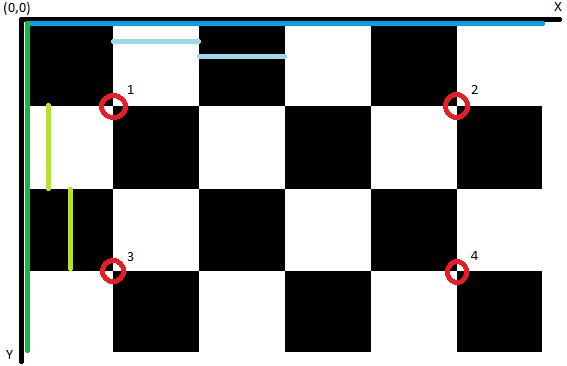
\includegraphics[scale=0.5]{bilder/schachbrett.png}
	\end{figure}

\end{frame}

%###########################

\begin{frame}{Kamera: Entzerrung}
Für die Kalibrierung des Kamerabildes mittels eines Patternmusters, muss zwischen zwei Ansichten unterschieden werde
	\begin{itemize}
		\item Weltkoordinaten = Patternkoords. ideal/entzerrt
		\item Bildkoordinaten = Patternkoords. aus aufgenommenem Bild/verzerrt
	\end{itemize}
\end{frame}

\begin{frame}{Kamera: Weltkoordinaten}
	Da die übergebenen Punkte nachher in ein 2D-Koordinatensystem, das vom Spiel, dargestellt werden sollen, werden die Erkennungspunkte des Schachbrettmusters als 2D-Punkte gespeichert:\\
	$WeltCoords = (x \cdot a, y \cdot a, 0)$\\
	$a$ = Kantenlänge, $x \in [0,Vert-1], y \in [0,Hort-1]$\\
\end{frame}

\begin{frame}{Kamera: Kalibrierungsparameter}
	\[s
	\begin{bmatrix}
	u\\v\\1
	\end{bmatrix}=
	\begin{bmatrix}
	f_{x} & 0 & c_{x}\\
	0 & f_{y} & c_{y}\\
	0 & 0 & 1
	\end{bmatrix}
	\begin{bmatrix}
	r_{11} & r_{12} & r_{13} & t_{1} \\
	r_{21} & r_{22} & r_{23} & t_{2} \\
	r_{31} & r_{32} & r_{33} & t_{3}
	\end{bmatrix}
	\begin{bmatrix}
	X\\Y\\Z\\1
	\end{bmatrix}
	\]
\end{frame}

\begin{frame}{Kamera: Kalibrierungsparameter}
	Eingabe:\\
	\begin{itemize}
		\item Bildkoordinaten 2D Matrix\\
		\item Weltkoordinaten 3D Matrix\\
		\item Anzahl vertikaler und horizontaler Fixpunkte im Schachbrett
	\end{itemize}
\end{frame}

\begin{frame}{Kamera: Kalibrierungsparameter}
	\begin{figure}[h]
		\centering
		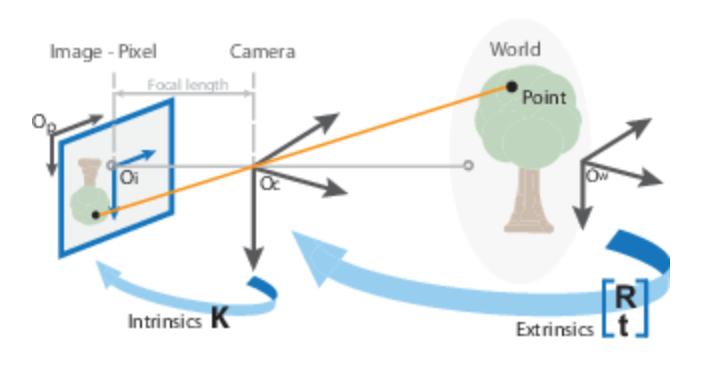
\includegraphics[scale=1.0]{bilder/extrinIntrin.PNG}
	\end{figure}
	Nun erhalten wir die extrinsischen, sowie die intrinsischen Entzerrungsparameter
\end{frame}

%###########################

\begin{frame}{Kamera: Mapping}
	Der letzte Abschnitt der Kamerakalibrierung stellt das Übertragen eines von der Queue-Erkennung gegebenen Punktes ins Spielfeld da. Um dies einwandfrei zu ermöglichen, müssen folgende Punkte erfüllt werden:
	\begin{itemize}
		\item[1.] äußersten Eckpunkte des, von der Kamera erfassten bilder bekannt sein\\
		$\implies$ die ganz äußersten Eckpunkte wie folgt berechnet werden:
		$\implies$ $Lila_{min} = Gruen_{min} - Rot_{min}$, $Lila_{max} = Rot_{max} - Gruen_{max}$
		\pause
	\end{itemize}	
\end{frame}

\begin{frame}{Kamera: Mapping}
		\begin{figure}[h]
		\centering
		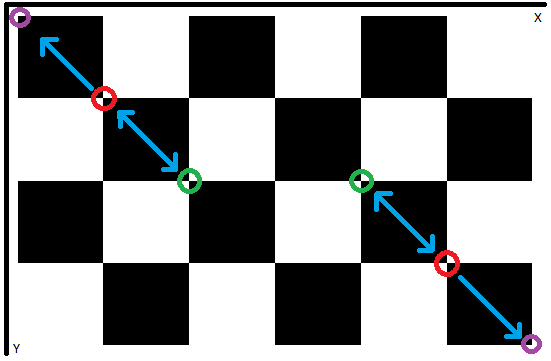
\includegraphics[scale=0.5]{bilder/schachbrettdiff.png}
		\caption{Schachbrettmuster Eckpunkte}
	\end{figure}
\end{frame}

\begin{frame}{Kamera: Mapping}
	Nun sind die äußersten Eckpunkte des Spielfeldes im Kamerakoordinatensystem bekannt und es ist möglich einen beliebigen 2D Punkt in das Spiel zu projizieren.
	
	$X \in [x_{min}, x_{max}]$ und $Y \in [y_{min},y_{max}]$ gilt.
	Sofern dies erfüllt ist, wird der gegebene Punkt mit folgenden Gleichungen jeweils mit der X- und Y-Koordinate umgerechnet :\\
	$X = \dfrac{(P.x - MIN.x) \cdot UR}{(MAX.x - MIN.x)}$, 
	$Y = \dfrac{(MAX.y - P.y) \cdot OL}{(MAX.y - MIN.y)}$
	
\end{frame}

\begin{frame}{Kamera: Mapping}
	\begin{figure}[h]
		\centering
		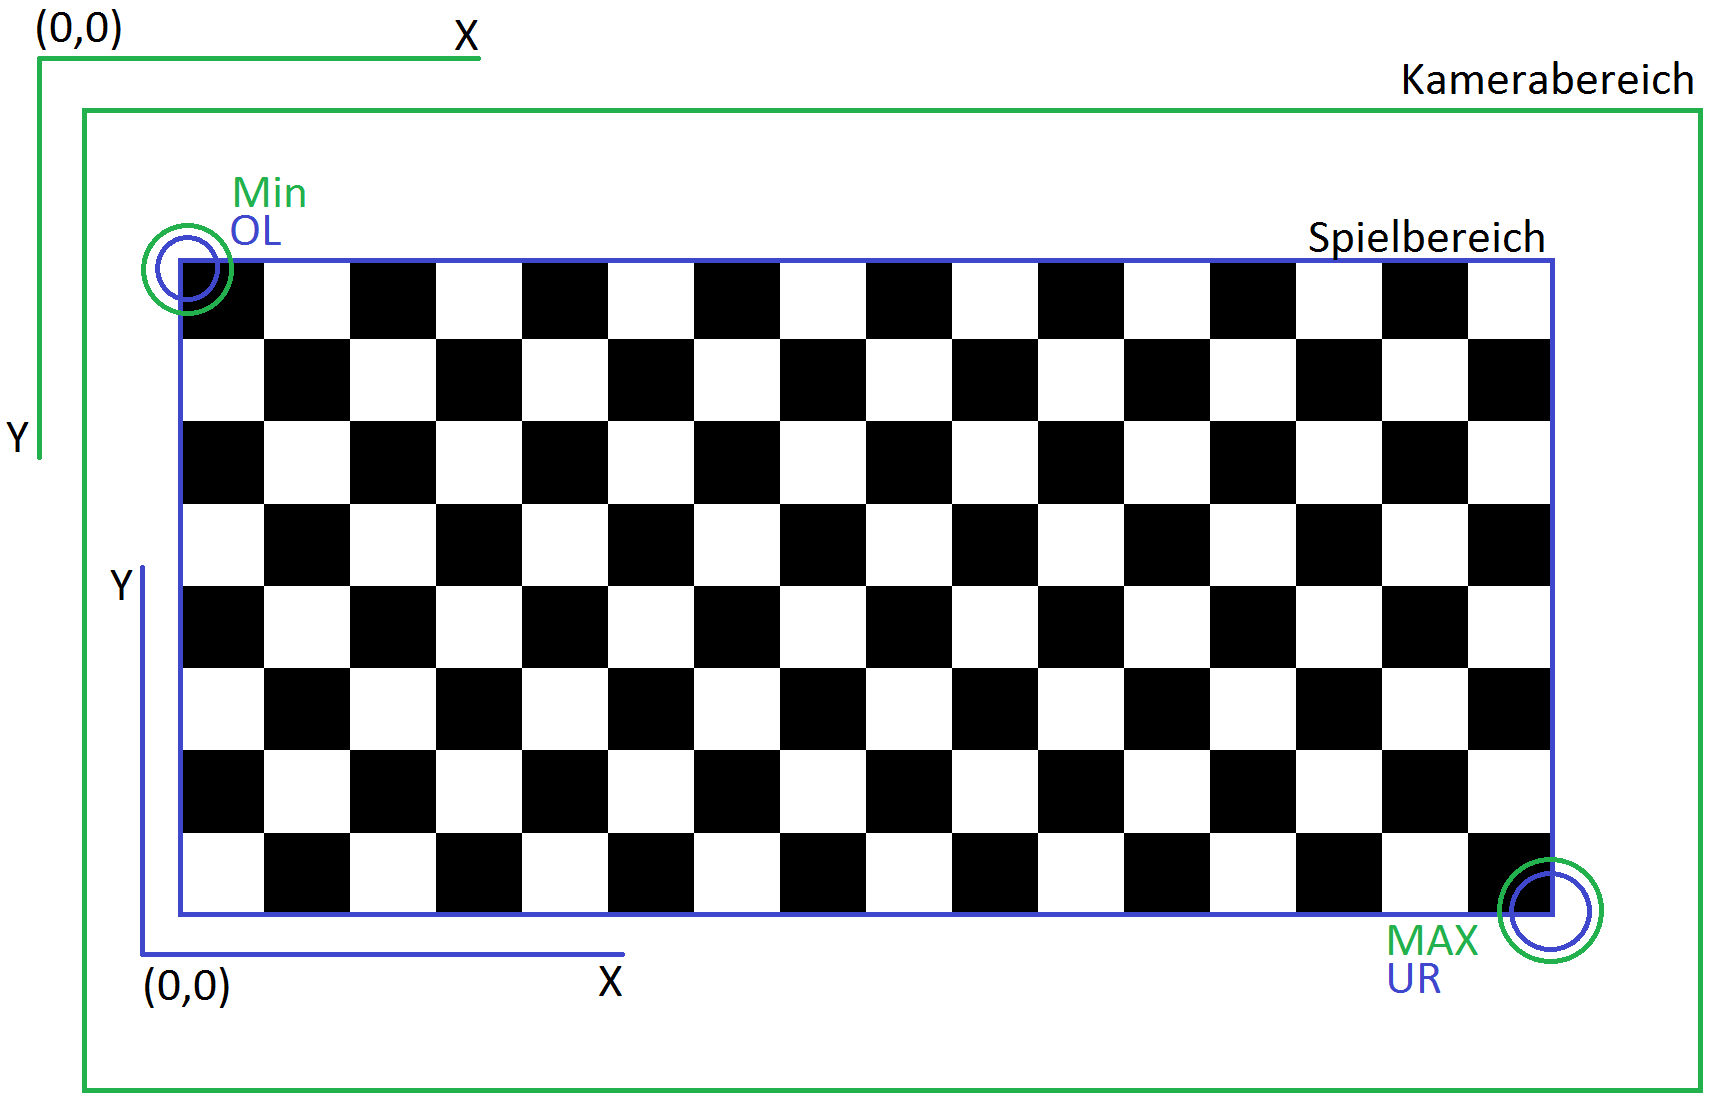
\includegraphics[scale=0.2]{bilder/schachbrettkamera.png}
		\caption{Kamera- und Spielkoordinatensystem}
	\end{figure}
\end{frame}